\documentclass[English,c,% 't' (resp. 'c') places text vertically at top/center of each slide
% PDF settings
hyperref={%
    pdftitle={FISA-DE2 OOP in Java},%
    pdfauthor={Muller, Gravier, Laforest, Subercaze},%
    pdfsubject={OOP in Java},%
    pdfkeywords={OOP, Java},%
    colorlinks=true,%
    urlcolor=blue,%
    linkcolor=%
    },%
% To load many pre-defined color names
xcolor={pdftex,svgnames} % dvipsnames, dvipsnames*, svgnames, svgnames*, x11names,
]{beamer}

\usetheme{Copenhagen}
%\setbeamertemplate{footline}[page number]
%\setbeamertemplate{frametitle}[default][center]
% To remove the navigation symbols from the bottom of slides:

% Remove navigation bar
\setbeamertemplate{navigation symbols}{}
% Remove outline at top
\setbeamertemplate{headline}{}

\addtobeamertemplate{navigation symbols}{}{%
    \usebeamerfont{footline}%
    \usebeamercolor[fg]{footline}%
    \hspace{1em}%
    \insertframenumber/\inserttotalframenumber
}

% Put text more on top of each slide for all slides
\addtobeamertemplate{frametitle}{}{\vspace*{-.7em}}

% Correct French/English indentation and splitting of words
\usepackage{babel}

% Correct management of accentuated chars in input file
\usepackage[utf8]{inputenc}

% Correct font for the generation of docs with accentuated chars
\usepackage[T1]{fontenc}      % Can handle hyphenation of words with accented characters
%%\usepackage[OT1]{fontenc}   % Might generated bad looking PDFs

% Insertion of images generated by external tools
\usepackage{graphicx}
% To generate pretty & scalable images directly in LaTeX
\usepackage{tikz}

% To print numbers correctly
\usepackage{numprint}

\usepackage[absolute,overlay]{textpos}

\usepackage{fourier}

\setbeamercovered{transparent}
\setbeamercovered{invisible}

\AtBeginSection[]
{
   \begin{frame}{Outline}
       \tableofcontents[currentsection]
   \end{frame}
}

\usepackage{url,manfnt}


% To be able to insert code listing
\usepackage{listings}

\definecolor{dkgreen}{rgb}{0,0.6,0}
\definecolor{gray}{rgb}{0.5,0.5,0.5}
\definecolor{mauve}{rgb}{0.58,0,0.82}

\lstset{frame=none,
  language=Java,
  aboveskip=1mm,
  belowskip=1mm,
  showstringspaces=false,
  columns=flexible,
  basicstyle={\tiny \ttfamily},
  numbers=left,
  numberstyle=\tiny\color{gray},
  keywordstyle=\color{blue},
  commentstyle=\color{dkgreen},
  stringstyle=\color{mauve},
  breaklines=true,
  breakatwhitespace=true,
  tabsize=2
}
\definecolor{algoTitle}{rgb}{0.84,0.83,0.94}

\usepackage{caption}
\DeclareCaptionFont{white}{\color{white}}
\DeclareCaptionFormat{listing}{\colorbox{algoTitle}{\parbox{\textwidth}{\bfseries #1#2 #3}}}
\captionsetup[lstlisting]{format=listing,labelfont=white,textfont=white}

\title[OOP in Java]{Object-Oriented Programming in \raisebox{-.3\height}{
\includegraphics[height=1.5em]{./images01/java_logo.png}}}
\logo{
\includegraphics[width=1cm]{images00/logo_tse.png}}
\author[Guillaume MULLER]{
  Guillaume \textsc{Muller}\\[1.2em]
  {\scriptsize \textit{based on work from:} \\[.1em]
    Ch. \textsc{Gravier}, F. \textsc{Laforest}, J. \textsc{Subercaze}}
}
\institute[TSE/UJM]{
  Télécom Saint-\'{E}tienne\\
  \medskip
  {\url{{pénom.nom}@univ-st-etienne.fr}}
}
\date[09/14/2020]{14~September~2020}

\begin{document}

%%%%%%%%%%%%%%%%%%%%%%%%%%%%%%%%%%%%%%%%%%%%%%%%%%%%%%%%%%%%%%%%%%%%%%
\begin{frame}
  \maketitle
\end{frame}

\section*{Git}
%%%%%%%%%%%%%%%%%%%%%%%%%%%%%%%%%%%%%%%%%%%%%%%%%%%%%%%%%%%%%%%%%%%%%%
\begin{frame}{Git \href{https://dzone.com/refcardz/getting-started-git}{[1]} \href{https://git-scm.com/book/en/v2}{[2]}}

{\scriptsize
  \begin{itemize}
    \item \textit{(Good way to create a portfolio)}
    \item Ditributed Management of source code files, diffs, versions\ldots{}
    \item Repository: local copy vs. centrally share repo
    \item Git manages only files, \textbf{not} (directly) directories
    \item To create a repository:\\
    \texttt{git init mylocalcopy/}
    \item To get an existing repository:\\
    \texttt{git clone https://the-repo-url}  \hfill \textit{From here, we are inside \texttt{mylocalcopy/}}
    \bigskip
%
    \item To tell git to manage a given file:\\
    \texttt{git add myfile.java}
    \item To check what git thinks of the files:\\
    \texttt{git status [myfile.java]}
    \item To tell git to ``store/accept'' the new version locally:\\
    \texttt{git commit -m "My message" myfile.java}
    \item To tell git to ``push'' the new version to everybody (remote):\\
    \texttt{git push}
    \item To get the lastest version from the others (remote):\\
    \texttt{git pull}
  \end{itemize}
}
\end{frame}


%%%%%%%%%%%%%%%%%%%%%%%%%%%%%%%%%%%%%%%%%%%%%%%%%%%%%%%%%%%%%%%%%%%%%%
\begin{frame}{GitLab \href{https://gitlab.com}{\color{white}{[1]}}}
  \begin{itemize}
    \item<1-> Create an account\\
    \url{https://github.com/join?ref_cta=Sign+up}
    \bigskip
%
    \item<2-> Create a project\\
    \onslide*<2>{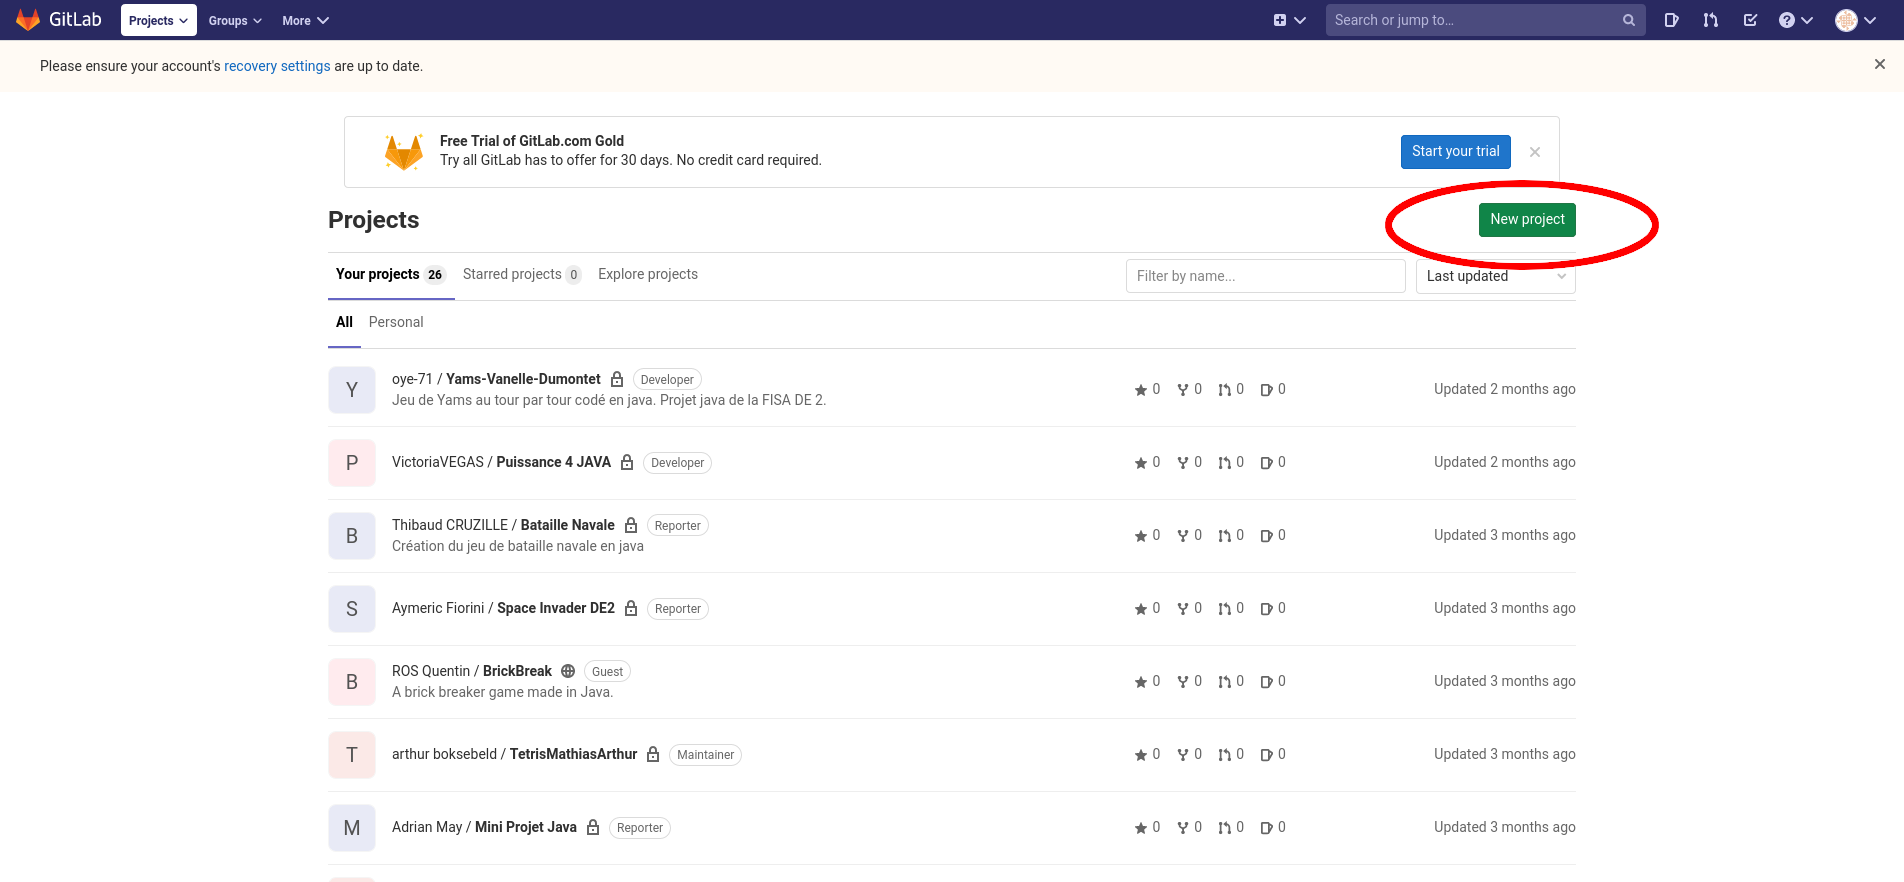
\includegraphics[width=.7\linewidth]{./images01/gitlab-create-project.png}}
    \onslide*<3>{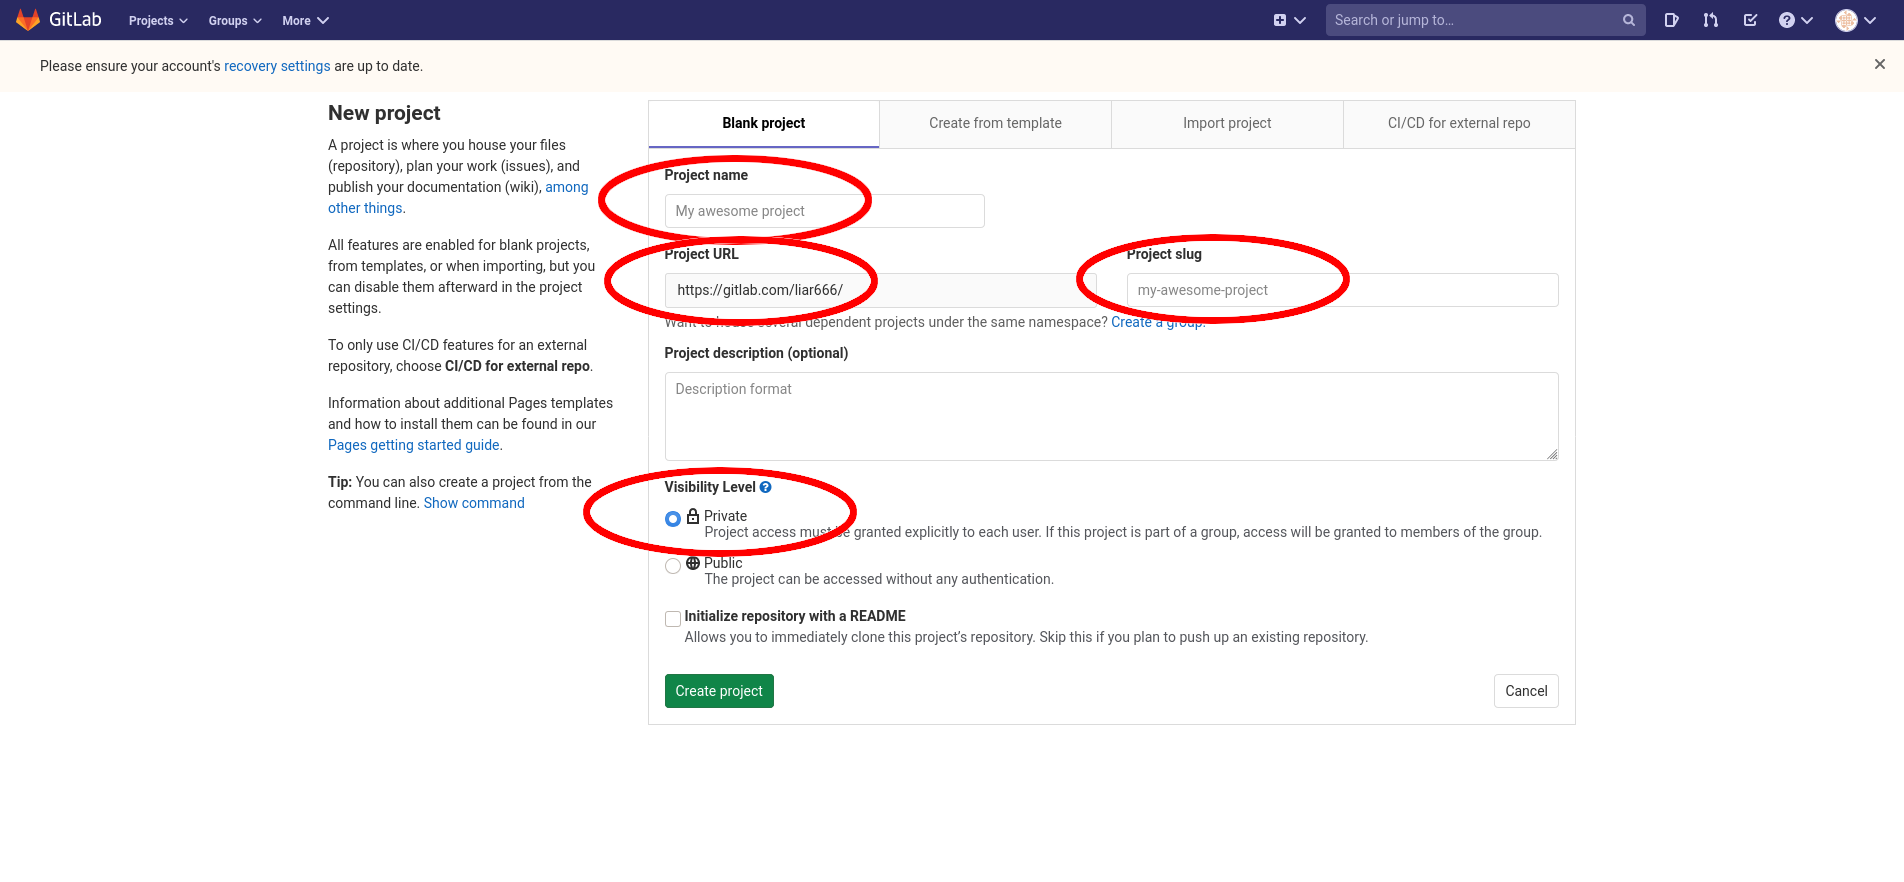
\includegraphics[width=.7\linewidth]{./images01/gitlab-create-project2.png}}
    \bigskip
%
    \item<4-> Get it:\\
    { \small
      \texttt{git clone https://gitlab.com/<user>/<project>}
    }
  \end{itemize}
\end{frame}

%%%%%%%%%%%%%%%%%%%%%%%%%%%%%%%%%%%%%%%%%%%%%%%%%%%%%%%%%%%%%%%%%%%%%%
\begin{frame}{GitHub \href{https://github.com}{\color{white}{[1]}}}
  \begin{itemize}
    \item<1-> Create an account\\
    \url{https://gitlab.com/users/sign\_in\#register-pane}
    \bigskip
%
    \item<2-> Create a project\\
    \onslide*<2>{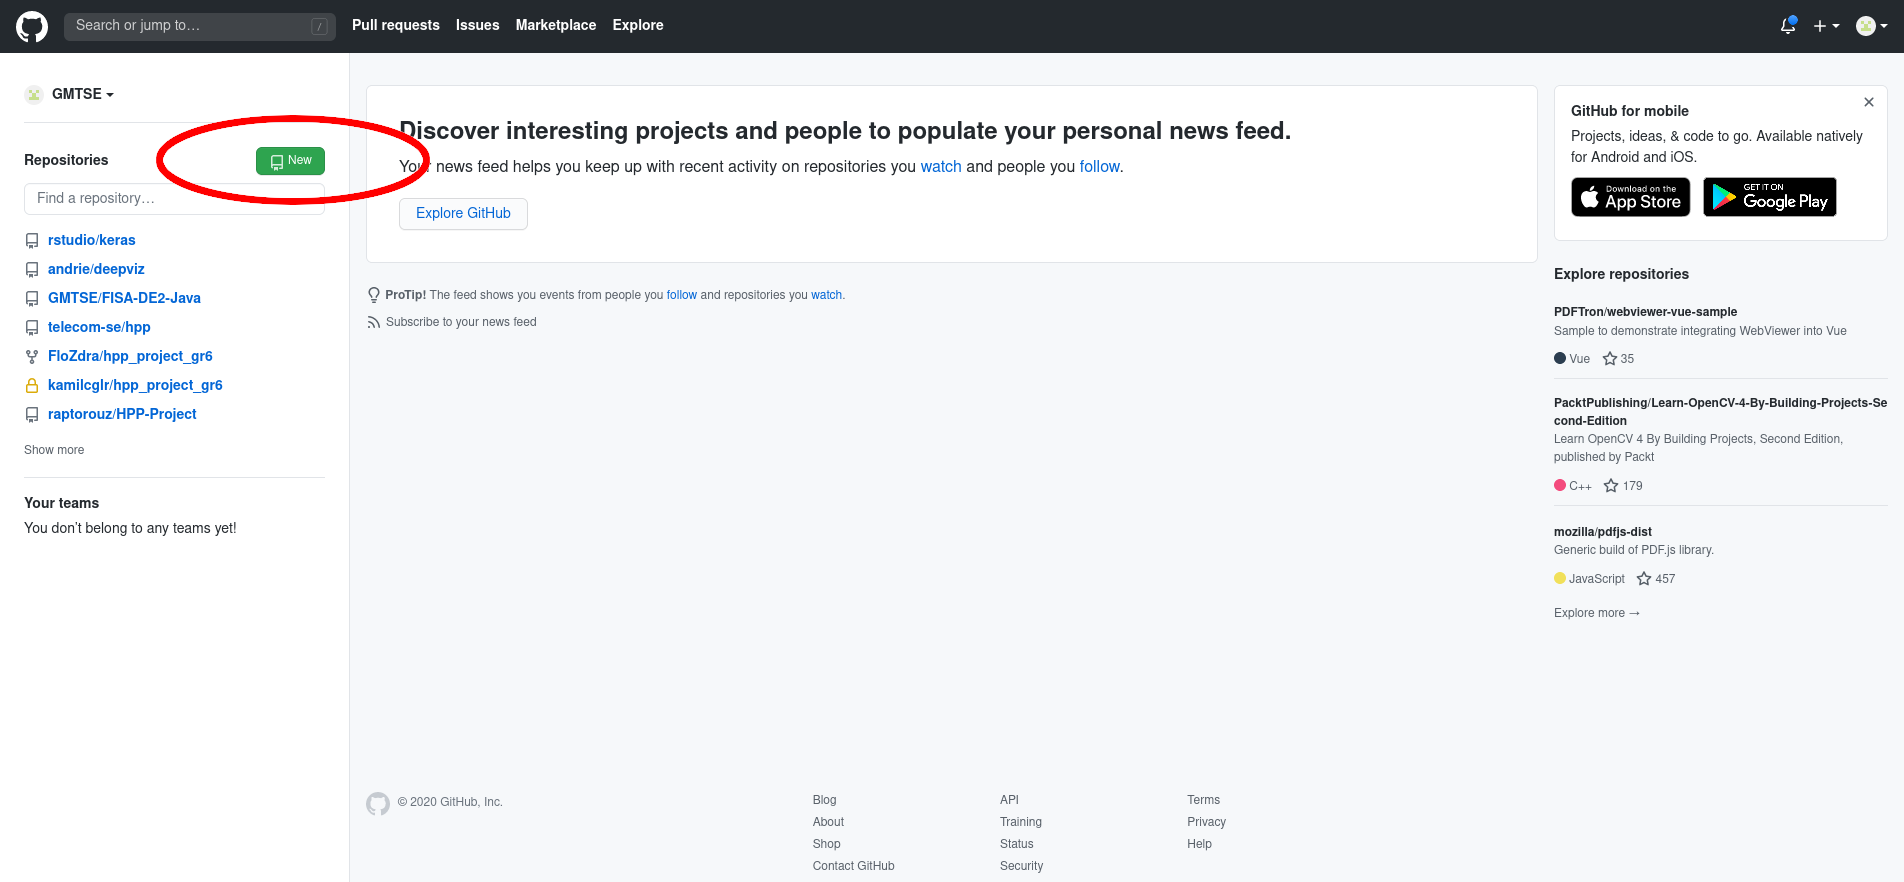
\includegraphics[width=.7\linewidth]{./images01/github-create-project.png}}
    \onslide*<3>{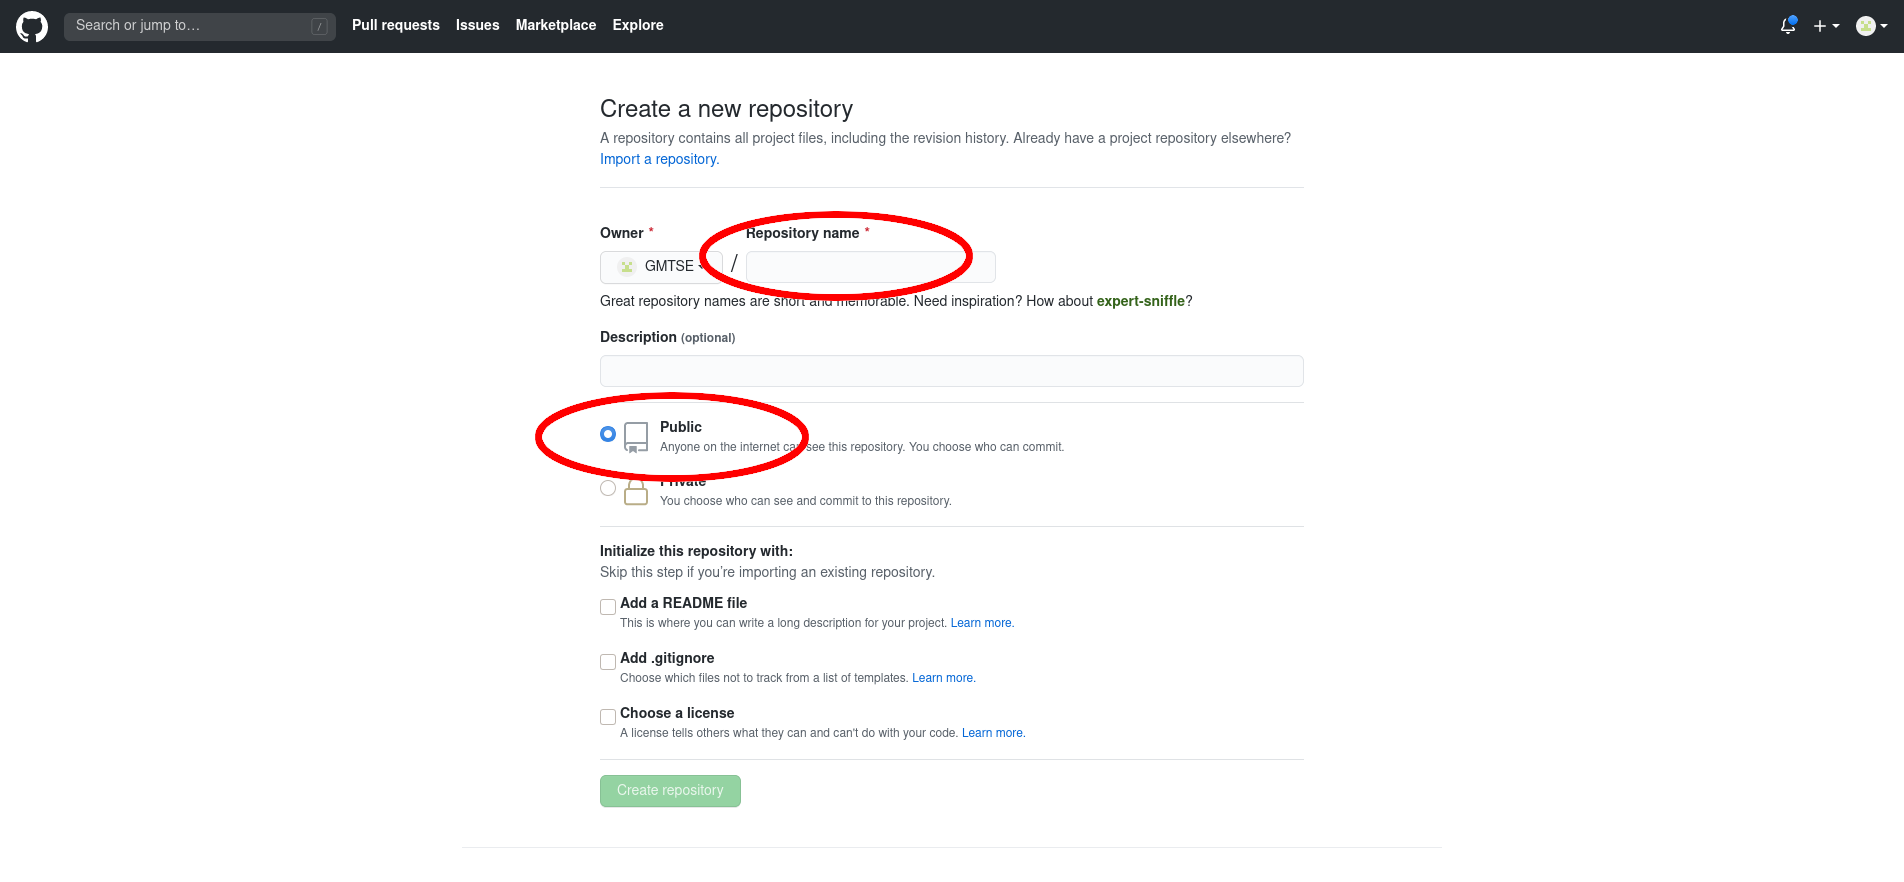
\includegraphics[width=.7\linewidth]{./images01/github-create-project2.png}}
    \bigskip
%
    \item<4-> Get it:\\
    { \small
      \texttt{git clone https://github.com/<user>/<project>.git}
    }
  \end{itemize}

\end{frame}

%%%%%%%%%%%%%%%%%%%%%%%%%%%%%%%%%%%%%%%%%%%%%%%%%%%%%%%%%%%%%%%%%%%%%%
\begin{frame}{Git with Eclipse}

  \begin{itemize}
    \item Install the eGit plugin
    \url{https://www.youtube.com/embed/WSdIbqw7Kz4}
    \bigskip
%
    \item Import the repository
    \url{https://www.youtube.com/embed/Fv_5KEN6Ix4}
    \bigskip
%
    \item Clone the content
    \url{https://www.youtube.com/embed/r77J-r0Pv74}
  \end{itemize}

\end{frame}

\end{document}
